\section{CONCLUSIONS AND FUTURE WORK} \normalfont

% \begin{dissQuote}{\~{}Margaret Boden, The Creative Mind: Myths and Mechanisms, pp. 58}
%     We all test the rules, and consider bending them; even a saint can appreciate science fiction. We add constraints (lucky numbers?), to see what happens then. We seek the imposed constraints (only two numbers to be added), and try to overcome them by changing the rules. We follow up hunches ('Let's do subtraction, too'), and - sometimes - break out of dead-ends. Some people even make a living out of pushing the existing rules to their limits, finding all the computational 'cans' that exist: creative tax-lawyers call them loopholes (and creative tax-legislators close them).
% \end{dissQuote}

\setlength{\epigraphwidth}{4in} 
\epigraph{We all test the rules, and consider bending them; even a saint can appreciate science fiction. We add constraints [...] to see what happens then. We seek the imposed constraints [...] and try to overcome them by changing the rules. We follow up hunches [...], and - sometimes - break out of dead-ends. Some people even make a living out of pushing the existing rules to their limits, finding all the computational 'cans' that exist: creative tax-lawyers call them loopholes (and creative tax-legislators close them)}{\textit{Margaret Boden \\ The Creative Mind: Myths and Mechanisms, pp. 58}}

% Final conclusions, what does your research means? 

% And now it begins. no, now it ends. 

%%%%%%%%%%%%%%%%%%%%%%%%%%%%%%%%%%%%%%%%%%%%%%%%%%%%%%%%%

This thesis explored~\acrshort{mi} collaboration between human designers and AI for the co-creation of games in~\acrshort{edd}, a~\acrshort{micc} system. The focus has been on developing techniques and algorithms to investigate this interaction to highlight and argue for the benefits that can be achieved. Specifically, mutual inspiration to explore unknown design areas, foster the designer's creativity, and establish adaptive experiences. Furthermore, the interaction between designers and AI arises multiple dynamic properties such as initiative, control, and expressivity. \emph{Initiative} relates to how either agent engages in the tasks and to what extent. \emph{Control} relates to the control mechanisms that are enabled for either agent to direct or constraint the output of the other agents based on some criteria. \emph{Expressivity} relates to the diversity of solutions that can be created by either agent.

% foster the designer's creativity and create adaptive experiences. Through these interaction and the approaches and algorithms proposed, this thesis have highlighted and argue the benefits that can be created. 

% In paper 1, the focus was on exploring the designer's impressions and requirements when using design tools. Paper 2 focused on giving explicit control to the designer over what to preserve in the~\acrshort{ea}. This allowed the computational designer to be more supportive by focusing on parts that the designer was not currently working on. Moreover, paper 3 introduced the~\acrlong{icmape}, an interactive version of the~\acrshort{mape} algorithm, one of the

One of the objectives of this thesis was on developing algorithms that could collaborate with designers, giving them a varying degree of control through control mechanisms while still being expressive (RQ1). Three control mechanisms were introduced where the designer had direct and indirect control over non-intuitive parameters of the~\acrshort{ea}. These were: \emph{Locking tiles}, \emph{designer's design}, and \emph{feature dimensions}. In \textsc{paper i} an explorative study was carried out to evaluate~\acrshort{edd} and it's current functionalities with game developers to gather and analyze game designer's requirements and impressions. \textsc{paper ii} focused on introducing aesthetic criteria to evaluate content, and as a way for the designer to preserve their content. The locking tiles feature was introduced, which allowed designers to designate areas of their design to be preserved by the~\acrshort{ea}. This allowed the computational designer to be more supportive by focusing on parts that the designer was not currently working on.

% that were a strong candidate to cope with both the control and expressivity dynamic properties that arose in the interaction.

Moreover, a strong candidate to cope with both the control and expressivity dynamic properties that arose in the interaction are~\acrshort{qd} algorithms. Thus, in \textsc{paper iii} it was introduced and implemented the~\acrlong{icmape}, a variation of the~\acrshort{mape} algorithm. Among its features, it enabled the designer to select feature dimensions (a key component of~\acrshort{mape}, explained in section~\ref{sec:map-elites}). The results from \textsc{paper iii} pointed towards enabling enough control since selecting feature dimensions and their granularity changes the search landscape and the retained solutions. However, this changes the features a designer might be interested on, but does not limit the expressivity of the algorithm to create diverse solutions. Further, the fitness function of~\acrshort{icmape} continuously adapts to the designer's design, acting as an indirect control mechanism.

The results from \textsc{paper iii} are further supported by preliminary results, where the behavior and generative space of~\acrshort{icmape} was analyzed by simulating design sessions. Given that one of the designer's interaction is the automated adaptation of the fitness based on the current design, we examined and evaluated how the search varied and adapted in a design session.
The results show that the algorithm adapts adequately and the designer has to some large extent, impact in the generative space with their design. More exciting is that~\acrshort{icmape} is able to explore new areas of the space through adapting to the designer's design without unexploring the other areas. This result can be seen in figure~\ref{fig:FigureRejectedPaper}. 

In short, controllability in many cases is a competing property with expressivity. Since the control and constraints that are imposed, usually limits the expressive range for any of the constrained agents. However, in this thesis we demonstrated that~\acrshort{qd} algorithms, specifically,~\acrshort{icmape} are able to cope with this, showing robustness, adaptability, and stability when interacted. It was provided meaningful control for the designer yet~\acrshort{icmape} adapted and kept exploring vast amounts of the generative space encountering high-performing solutions. 

\begin{figure}[t]
\centerline{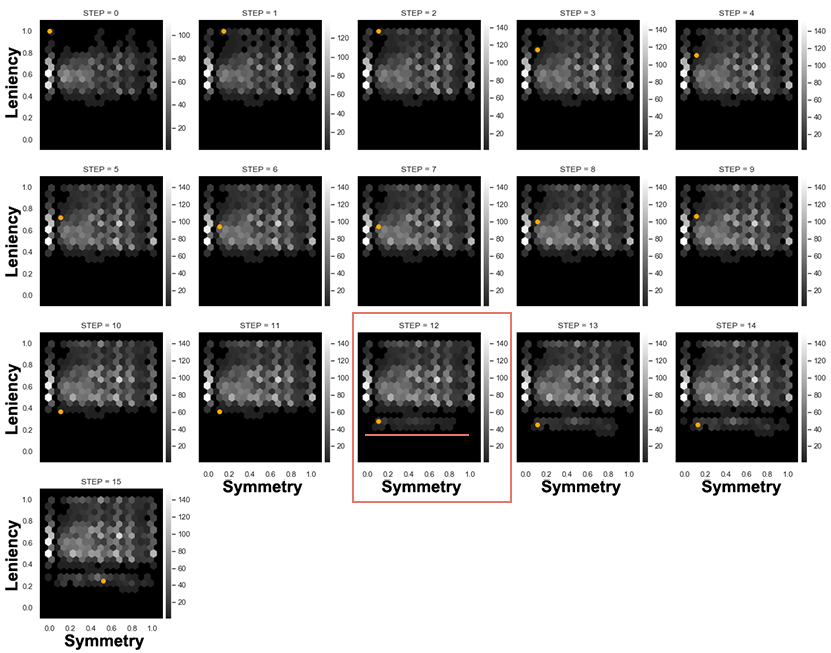
\includegraphics[width=\textwidth]{figures/ICMAPE-figs/accumulative__X-sym-Y-len-2.png}}
%\centerline{\includegraphics[width=0.55\textwidth]{figures/low-len/accu__X-sym-Y-len.png}}
\caption{Aggregated Expressive Range Analysis using Symmetry and Leniency as feature dimensions. The orange dot represents the designer's design that each step is edited and moving in the generative space. In step 12, it is highlighted the step when the designer's design enters a new generative area, which helps~\acrshort{icmape} explore the new area.}
\label{fig:FigureRejectedPaper}
\end{figure}

% However, in this thesis it was provided meaningful control for the designer 

% However,~\acrshort{qd} algorithms, specifically,~\acrshort{icmape} has provided meaningful control for the designer over the generation process  was seen as a competing

% seamlessly competing properties such as control and expressivity due to the control and constraints imposed from one side to the other could limit the expressivity of the other



% The designer was given explicit control over what to 

% In \textsc{paper ii}, the locking tiles ability was introduced, which allowed the designer to designate areas of their design to be preserved by the~\acrshort{ea}. 

% ~\acrshort{qd} algorithms is a family of algorithms that were a strong candidate to cope with both this control and expressivity aspect.

% Along with these approaches, the fitness function of~\acrshort{icmape} continouusly adapts to the designer's design, acting as an indirect control mechanism. In short, three control mechanisms were introduced where the designer had direct and indirect control over non-intuitive parameters of the~\acrshort{icmape}. These were: \emph{Locking tiles}, \emph{designer's design}, and \emph{feature dimensions}.


% This is further supported by preliminary results where it was analyzed~\acrshort{icmape} behavior and generative space in relation a design session simulation. Given that one of the designer's interaction is the automated adaptation of the fitness based on the current design, we examined and evaluated how the search varied and adapted in a design session. Our preliminary results show that not only the algorithm adapts adequately and the designer has to some large extent, impact in the generative space of the algorithm, but that~\acrshort{icmape} is able to explore new areas of the space through adapting to the designer's design without unexploring the other areas. Such a phenomenon can be seen in figure~\ref{fig:FigureRejectedPaper}

% Such a phenomenon can be seen in figure~\ref{fig:FigureRejectedPaper}


% While paper 1, 2, and 3, focused on the generative aspect of the computational designer and alternating control mechanisms for the designer, paper 4, 5, and 6 focused on creating player and designer models to create adaptive experiences. In paper 4 --- , in paper 5 and 6 the focus was on ... 

Moreover, the work in \textsc{paper i, ii, ii} and the interest on seeking alternative approaches to foster creativity, to create adaptive experiences, and to enable more autonomy and initiative for the AI, directed the research towards player and designer modeling. The former, was explored in \textsc{paper iv}, where personality-driven player models were created to investigate their usability as a representative surrogate model and possible complement value in gameplay. 

% Designer Modeling was explored through \textsc{paper v, vi}.
\textsc{paper v} and~\textsc{paper vi} presented examples of designer modeling by modeling different designers' procedures. These could be used as surrogate models to enhance the understanding on design processes and the usability of design tools, such as~\acrshort{edd}. \textsc{paper v} presented a clear artifact design used to steer the generation of new suggestions based on the \textit{in situ} created preference model. This work demonstrated the benefits that come with integrating these models in the~\acrshort{mi} loop such as the possibility of seemlessly creating preferred content. However, it also demonstrated the challenges such as selecting and collecting representative data or training-and-using models as designers develop. Furthermore,~\textsc{paper vi} presented the development of a novel model to analyze the designer's design process, which could inform generative processes on the style, goal, and intentions of the designer. The anylisis of the resulting clusters based on the design process each designer used, resulted in the designer personas. This designer personas was presented as archetypical paths taken by designers through the clustered style space. Both models allow for the analysis of design and creative processes from an abstract level rather than specific steps, akin to procedural personas or game design patterns. 


% thus, allowing for 

% it can be used to  routes designers take 


% the designer personas described in \textsc{paper vi} present an analysis 

% lacking it's implementation and test. However, designer personas usability in practice is discussed as it could be used to adapt the content generated by other techniques such as~\acrshort{icmape}. 

These approaches towards designer modeling have shown the capabilities of modeling several procedures and how could they be used. They also show that design processes can be analysed in a more abstract level yielding interesting similarities among seamlessly different designers or design processes. Designer modeling has the possibility to create adaptive experiences for individual or group of designers, and could enable more autonomy and initiative for the AI. However, whereas this, and its usability as surrogate models to enhance the collaboration, interaction, and generation produce actual benefits to the dynamic workflow of~\acrshort{micc} tools remains open for exploration, as a promising area.

% If the aim of this research area is to push harder for mixed-initiative tools, where more autonomy is given to the AI, and for humans to consider the AI as a colleague as described by Lubart~\cite{LUBART2005-computerPartners} and Guzdial et al.~\cite{Guzdial2019-AISystemDesign-Creators} that can be taken serious and used its input as a key factor in the development of any type of content. Then we are required to develop AIs and tools that not only provides interesting and valuable input to the human, but also adaptive experiences that 


% \textsc{paper v, vi} present approaches towards designer modeling in a~\acrshort{micc} environment. 

% These approaches towards designer modeling are a promising area that would enable 

% Whereas modeling designer's procedures as described in~\cite{Liapis2013-designerModel}, and its usability as surrogate models to steer the collaboration and interaction produce actual benefit to the dynamic workflow of~\acrshort{micc} tools remains open for exploration, as a promising area.


% and \textsc{paper vi}. 

% Moreover, the work from \textsc{paper i, ii, ii}, the objective to explore~\acrshort{mi} interaction, and alternative approaches to foster creativity, create adaptive experiences, and enable mo

% Moreover, the work in paper 1, 2, and 3, and our aim to explore interaction, control mechanisms, and other ways to foster the creativity, create adaptive experiences, and enable more autonomy and initiative from the AI. Directed the research towards player modelign and designer modeling. The former, explored thoruhg paper 4, personality-driven player models were created and it was investigated it's usability as a representative player model and possibhle complement value. The latter, designer modeling, was explored through paper 5 and paper 6

% \textsc{paper iv} and~\textsc{paper vi} presented examples of designer modeling by modeling different designers' procedures and design processes, which could be used as surrogate models to enhance the understanding on design processes and the usability of design tools, such as~\acrshort{edd}. \textsc{paper v} presented a clear artifact design used to steer the generation of new suggestions based on the \textit{in situ} created preference model, while~\textsc{paper vi} presents the development of a novel model to analyze the designer's design process lacking it's implementation and test. However, designer personas usability in practice is discussed as 

% Three control mechanisms were introduced where the designer had direct and indirect control over non-intuitive parameters of the~\acrshort{icmape}. These were: \emph{locking tiles}, \emph{designer's design}, and \emph{Feature dimensions}

% When designers and AI engage in this interaction, multiple dynamic properties arise such as initiative, control, and expressivity. \emph{Initiative} relates to how either agent engages in the tasks and to what extent. \emph{Control} relate to the control mechanisms that are enabled for either agent to direct or constraint the output of the other agent based on some criteria. \emph{Expressivity} relates to the diversity of solutions that can be created by either agent. One of the objectives of this thesis was on developing algorithms that could collaborate with designers, giving them a varying degree of control through control mechanisms


% These dynamic properties are examined and evaluated in relation to 

% The focus was on developing algorithms that could not only allow more expressive content generation, but also that allowed a varying degree of control for the designer.


% also point out that the results from paper 3 point out towards enabling enough control since selecting feature dimensions and their granularity changes the search landscape and the retained solutions. However, this just change the interested features a designer might be interested on, and does not limit the expressivity of the algorithm to create diverse solutions. This is further supported by preliminary results of an unpublished study where we analyzed~\acrshort{icmape} behavior and generative space in relation to a simulation of a design session. Given that one of the designer's interaction is the automated adaptation of the fitness based on the current design, we examined and evaluated how the search varied and adapted in a design session. Our preliminary results show that not only the algorithm adapts adequately and the designer has to some large extent, impact in the generative space of the algorithm, but that~\acrshort{icmape} is able to explore new areas of the space through adapting to the designer's design without unexploring the other areas. Such a phenomenon can be seen in figure~\ref{fig:FigureRejectedPaper}


% This thesis has explored the interaction between human designers and AI to co-create games in~\acrshort{edd}, a~\acrshort{micc} system. By engaging in this mutual feedback loop, this thesis examined the properties and dynamics 

% Through this interaction, this thesis examined the properties and dynamics that arose when giving control mechanisms to the designer.

% Moreover, the work in paper 1, 2, and 3, and our aim to explore interaction, control mechanisms, and other ways to foster the creativity, create adaptive experiences, and enable more autonomy and initiative from the AI. Directed the research towards player modelign and designer modeling. The former, explored thoruhg paper 4, personality-driven player models were created and it was investigated it's usability as a representative player model and possibhle complement value. The latter, designer modeling, was explored through paper 5 and paper 6

% This thesis has explored the properties of~\acrshort{mi} collaboration, specifically for the co-creation of games. The focus was on developing techniques and algorithms to investigate the interaction between designers and AI to foster the designer's creativity and create adaptive experiences. 

% In paper 1, the focus was on exploring the designer's impressions and requirements when using design tools. Paper 2 focused on giving explicit control to the designer over what to preserve in the~\acrshort{ea}. This allowed the computational designer to be more supportive by focusing on parts that the designer was not currently working on. Moreover, paper 3 introduced the~\acrlong{icmape}, an interactive version of the~\acrshort{mape} algorithm, one of the

% While paper 1, 2, and 3, focused on the generative aspect of the computational designer and alternating control mechanisms for the designer, paper 4, 5, and 6 focused on creating player and designer models to create adaptive experiences. In paper 4 --- , in paper 5 and 6 the focus was on ... 

% The focus was on developing algorithms that could not only allow more expressive content generation, but also that allowed a varying degree of control for the designer. Through this,  

% in a ~\acrshort{micc} tool called~\acrlong{edd}. Through 

% This thesis explored  interaction in mixed-initiative scenarios, specifically for the creation of games in~\acrshort{micc} tool called~\acrlong{edd}.

\subsection{Future Work}

This thesis dived into the essential question of how to create tools where human designers can have a \emph{colleague} partnership and collaboration with the AI, the properties that arise from this, and ways to enhance the collaboration, several if not more areas remain open. 
% While the work in this thesis has explored the interaction between human designers and AI, the properties that arise from this, and ways to enhance the collaboration, several if not more areas remain open. 

For instance, \textsc{RQ1} was partially addressed by introducing and implementing~\acrshort{icmape} in~\acrshort{edd}. However, it is necessary to examine the behavior of~\acrshort{icmape} when used for this interaction. These behaviors could be: how the generative space is affected by the design sessions, the combination with designer modeling, or how dynamic feature dimensions (e.g., similarity and inner similarity) affect the expressiveness of the algorithm.~\acrshort{pcg} through~\acrshort{qd} was proposed recently~\cite{gravina2019procedural}, pointing towards the interesting avenues that are approaching, and as discussed in this thesis, the many possibilities they have when introduced in human-AI interaction and collaboration.

Furthermore, it has been proposed two approaches to model different designer procedures as designer modeling but more work needs to be in place to operationalize the findings and models. For instance, how to use and transform the designer personas and the design style clustering presented in \textsc{paper vi} into an applicable model to study designers and their design and creative process. Moreover, how to use these models to steer the generation of content and create adaptive experiences remains open, as the interaction with designers is dynamic and heterogeneous.

% In addition to exploring more in depth the RQs presented in this thesis,

\subsubsection{Explainable AI}

Moreover, to establish an in-depth relationship between human and AI, trustworthiness is also required from the AI, in order to give more autonomy, responsability, and initiative to the AI in creative tasks. Explainable AI is a research field that aims at increasing the transparency of AI systems, making AI systems more accessible, and more understandable~\cite{adadi2018peeking,Doshi-Velez2018}.

% However, explanations should be aligned with the users' understanding to don't hinder the usability of systems, as demonstrated by Nourani et al.~\cite{Nourani2019-meaningfulExplanations}, who discuss the effects of meaningful and meaningless explanations to users of an AI interactive systems.

Zhu et al.~\cite{Zhu2018-XAIDesignersMICC} proposed the field of eXplainable AI for Designers (XAID) as a human-centered perspective on MI-CC tools. This work discusses three principles of mixed-initiative, \emph{explainability}, \emph{initiative}, and \emph{domain overlap}, where the latter focuses on the study of the overlapping creative tasks between game designers and black-box PCG systems in mixed-initiative contexts. This work deems of high relevance the inclusion of data-driven and trained artifacts to facilitate a fluent bi-directional communication of the internal mechanisms. An example of this is presented by Xie et al.~\cite{xie2019interactive}, where they explored visualization techniques through an interactive level designer tool called \textit{QUBE} to explain and introduce machine learning principles to game designers.


% Aim at how to operationalize our findings and models, such as the designer personas and the design style clustering~\cite{alvarez2020-designerpersonas}, into an applicable model that can be used to study how designers move through the design style space and steer with that the generation of the~\acrshort{icmape}. Through this, we expect to get a deeper and more extensive dive into exploring RQ3 and RQ4, concluding with a more informed guess into what type of data is needed and how to collect it for RQ2. 


% Further,~\acrshort{icmape} is one algorithm within the~\acrshort{qd} paradigm that could be used to explore~\acrshort{micc} interaction.

% through~\acrshort{icmape}, it was partially addressed RQ1, but examining the extent of~\acrshort{qd} algorithms 

% This thesis has explored the interaction between human designers and AI 

% I am missing to bring interpretable and explainable AI to the scene!~\cite{Doshi-Velez2018,Zhu2018-XAIDesignersMICC,Nourani2019-meaningfulExplanations,OPAQUEAI,TransparencyGUidelines,explanatoryML}

% While they are all related to the context of dungeon and adventure games, there are two dimensions, \emph{similarity} and \emph{inner similarity}, which adapts dynamically to the current, i.e., at different time-steps, it will yiled

\subsubsection{Holistic Procedural Content Generation}

An interesting and exciting path would be to explore the concept of holistic~\acrshort{pcg} and orchestration of the different game facets~\cite{Liapis2019-OrchestratingGames} in connection with the~\acrshort{mi} paradigm. Holistic~\acrshort{pcg} is the generation of multiple content (in different game facets) fitting each other in harmony as a collaborative process akin to how games are developed, with a limited amount of examples, but exhibiting generative results with exciting results~\cite{hartsook2011-storyWorlds,Cook2014-ARogueDream,hoover2015-audioinspace,Smith2011-situatingQuests,dormans2011generating}. However, to what extent the generation is created in such a harmony that the facets interact and affect each other, and to what degree the user has the means to interact with it is an open area for active research. 

Furthermore, there exist an essential link and relation between space (e.g., level or objects within) and narrative (e.g., the story tried to be told); thus, choosing and associating level design and narrative as two facets to explore within the holistic~\acrshort{pcg} approach is appropriated. This was presented and described by Kybartas and Bidarra's survey~\cite{kybartas2016survey}, and explored and supported by related work~\cite{aarseth2005hunt,Dehn1981-StoryGen,Lebowitz83-CreatingStorytelling,hartsook2011-storyWorlds,Karavolos2015-miccMissionsLevels,abuzuraiq2019-taksim}.

Thus far, some exploratory work has been done in combining both facets in the generative process of~\acrshort{edd}. Firstly, through a simple but effective way of analyzing patterns and objectives created by designers when designing their levels~\cite{flodtol2020-WIPMakeSenseDungs}, and secondly, by introducing~\acrshort{mi} creation of quests using grammars to compose a series of subsequent objectives together with the designer~\cite{grevols2020-BS}. 

Therefore, having this as a base and using the current findings in this thesis, the aim is to explore the~\acrshort{micc} paradigm applied to holistic~\acrshort{pcg} through the following RQ and subRQs (continuing the numbering from the RQs presented in this thesis): 



% Furthermore, there are even less examples combining such a concept with~\acrshort{micc}~\cite{Karavolos2015-miccMissionsLevels,abuzuraiq2019-taksim}. 

% we aim to explore the~\acrshort{micc} paradigm applied to holistic~\acrshort{pcg} through the following RQ and subRQs (continuing the numbering from the RQs presented in this thesis):

% . There is a limited amoThe examples that with not many examples but with outstanding results exhibiting such generation

\begin{itemize}
    \item[] \textbf{RQ4.} How can level design and narrative interact, act as constraints, be intertwined, and in general, have an active role affecting each other, in order to, produce a holistic system?
    \begin{itemize}
        \item[] \textbf{RQ4.1:} What are the requirements and main factors needed to establish a relation between the level design and the narrative, and what are the criteria to evaluate the respective generated content? 
        \item[] \textbf{RQ4.2:} What are the factors to be considered when implementing such a paradigm and system in a mixed-initiative application, where a designer will be able to interact with the content?
        \item[] \textbf{RQ4.3:} What are the effects of producing and using a holistic system for the creative process of a designer, and what challenges are imposed on computational creativity? 
    \end{itemize}
\end{itemize}

% Presented and described by Kybartas and Bidarra's survey~\cite{kybartas2016survey}, and based on 

% described by Kybartas and Bidarra survey on narrative techniques~\cite{kybartas2016survey} and pointed out  

% Combining level design and narrative is not a random choice, rather 

% Discuss more into this:~\cite{Kreminski2018-SketchingStorylets,Garbe2019-StoryletsAssembler}

% Kybartas and Bidarra presented a survey on narrative techniques~\cite{kybartas2016survey}
% There exists an essential link and relation between narrative and space, as some discuss that narrative is a consequence and dependant on the~\cite{Barthes1966-structurenarr,abbott2002-narrative,chatman1980-storyDiscourse,aarseth2005hunt,Dehn1981-StoryGen,Lebowitz83-CreatingStorytelling}
% Narrative has an essential link and relation to 

%in the shape of bachelor theses from some of my students, exploring ways of integrating generation of narrative as objectives and quests in the~\acrlong{edd}. 

\subsubsection{Exploring Agency and Initiative in Mixed-Initiative}

Moreover, as it is explored paths towards adaptive experiences that recognize several designer procedures; it is expected to establish the foundations of a deeper relation between human and AI. Through this thesis, control mechanisms were given to designers while not reducing the expresiveness of the AI. Further, examining and modeling different designer procedures such as their design process, style, preferences, and goals as they create content, have enabled this thesis to explore important steps towards a mature relationship. However, this thesis barely scratched the surface of the relationship, the possibilities that emerge with them, and the initiative and role of the AI. It is hypothesised that this is needed to create more autonomy and initiative for the AI, and to establish a trustworthy relationship between both agents, yet, this might not be enough. Therefore, another future direction is to explore varying autonomy, agency, and initiative for both agents and how that affect the interaction and design and creative process of the co-design and~\acrshort{mi} paradigm. This is compiled into the following RQ:


% is how varying the autonomy, agency, and initiative of t

\begin{itemize}
    \item[] \textbf{RQ5.} How does the agency of the designer and the agency of the computational designer in mixed-initiative approaches, and the interaction between both actors, affects the overall design process and the usefulness of mixed-initiative tools?
\end{itemize}

% Finally, it is exciting to have explored all that this thesis present, but it is even more to see the road in front and realize all the paths that remain open and to be explored through future work.


% while this thesis has presented steps towards a better understanding through designer modeling and , it is especulated this thesis only especulates  has explored speculates that both of these research areas are needed to establish a trust relationship between both actors, yet, this might not be enough.

% Giving control to the designer while not reducing the expressive power of the AI, understanding different designer procedures such as their design process, style, and goals as they create levels, and modeling multiple subjective properties such as designers preferences and intentions; have enabled this thesis to explore interesting and important steps towards a mature relation. However, this thesis barely scratched the surface of the relationship and the possibilities that emerge with them. 

% Moreover, as it is explore paths towards adaptive experiences that recognize several designer procedures; we hope to establish the foundations of a deeper relation between human and AI. Giving control to the designer while not reducing the expressive power of the AI, understanding different designer procedures such as their design process, style, and goals as they create levels, and modeling multiple subjective properties such as designers preferences and intentions; have enabled this thesis to explore interesting and important steps towards a mature relation. However, this thesis barely scratched the surface of the relationship and the possibilities that emerge with them. 

% Moreover, as introduced in the problem statement (see section~\ref{sec:problemst}), it is required to have both an understanding from the AI of the multiple human procedures and an understanding from the human of how the AI system operates and it's decision process. In this thesis, this has been used and explained as Designer Modeling~\cite{Liapis2013-designerModel} and Explainable AI~\cite{Zhu2018-XAIDesignersMICC}. However, while this thesis has presented steps towards a better understanding through designer modeling, it is especulated this thesis only especulates  has explored speculates that both of these research areas are needed to establish a trust relationship between both actors, yet, this might not be enough. There are 


% As introduced in the problem statement (see section~\ref{sec:problemst}), it is required to have both an understanding from the AI of the multiple human procedures and an understanding from the human of how the AI system operates and it's decision process,  which translates to Designer Modeling~\cite{Liapis2013-designerModel} and Explainable AI~\cite{Zhu2018-XAIDesignersMICC}. However, such a system does not exist, and this thesis speculates that both of these research areas are needed to establish a trust relationship between both actors, yet, this might not be enough. There are 

% \begin{itemize}
%     \item[] \textbf{RQ5.} How does the agency of the designer and the agency of the computational designer in mixed-initiative approaches, and the interaction between both actors, affects the overall design process and the usefulness of mixed-initiative tools?
% \end{itemize}

% It is exciting to have explored all this thesis present, but it is even more to see the road in front and realize all the paths that remain open and to be explored through future work.